\section{Web crawling}
\textbf{Web crawling} is the process by which we \textbf{gather pages from the Web}, in order to index them and support a search engine. The objective of crawling is to \textbf{quickly} and \textbf{efficiently} gather as \textbf{many useful web pages as possible}, together with the link structure that interconnects them. 

The goal of this chapter is not to describe how to build the crawler for a full-scale commercial web search engine. We focus instead on a range of \textbf{issues} that are generic to \textbf{crawling} from the student project scale to substantial research projects. 

\subsection{Features}
We now list some features that a web crawler must provide:

\begin{itemize}
    \item \textbf{Robustness}: the Web contains servers that create spider traps, which are generators of web pages that mislead crawlers into getting stuck fetching an infinite number of pages in a particular domain. Crawlers must be designed to be \textbf{resilient} to such \textbf{traps};
    \item \textbf{Politeness}: a crawler must \textbf{respect} both the implicit and the explicit \textbf{policies} (i.e. specifications on which portions of a site can be crawled) of Web servers regulating the rate at which a crawler can visit them. 
\end{itemize}

Other features that a Web crawler should provide are:

\begin{itemize}
    \item \textbf{Distributed}, i.e. it should be designed to run on multiple distributed machines;
    \item \textbf{Scalable}, i.e. it should be designed to increase the crawl rate by adding more machines;
    \item \textbf{Performance and efficiency}, i.e. it should permit full use of available processing and network resources;
    \item \textbf{Quality}, i.e. the crawler should be biased towards fetching "useful" pages first;
    \item \textbf{Extensible}, i.e. it should be adaptable to new data formats and protocols;
    \item \textbf{Freshness}, i.e. it should continue fetching fresh copies of a previously fetched page.
\end{itemize}

\subsection{Crawling}
The basic operation of any hypertext crawler is as follows. 

\begin{enumerate}
    \item The crawler begins with \textbf{one or more URLs} that constitute a \textbf{seed set};
    \item It picks a \textbf{URL} from this seed set, then \textbf{fetches} the web page at that URL;
    \item The fetched page is then parsed, to extract both the \textbf{text} and the \textbf{links} from the page (each of which points to another URL). 
    \begin{itemize}
        \item The extracted text is fed to a \textbf{text indexer};
        \item The extracted links (URLs) are then added to a \textbf{URL frontier}, which at all times consists of URLs whose corresponding \textbf{pages} have \textbf{yet to be fetched} by the crawler. Initially, the URL frontier contains the seed set; as pages are fetched, the corresponding URLs are deleted from the URL frontier.
    \end{itemize} 
\end{enumerate}

A visual representation of the seed set and the frontier is provided in Picture \ref{crawling}: as we can see, there are many crawlers that get the URL from the frontier, implemented as a queue.

\begin{figure}[h!]
		\centering
		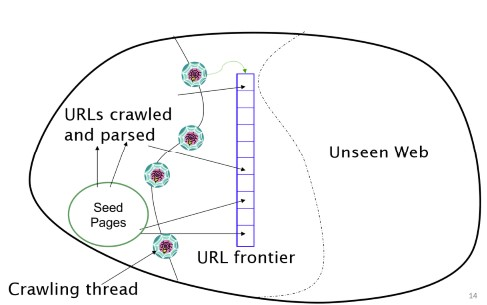
\includegraphics[scale = 1.6]{img/crawling.jpg}
		\label{crawling}
        \caption{Visual representation of the crawling process}
\end{figure}

This seemingly \textbf{simple recursive traversal} of the web graph is \textbf{complicated} by the many \textbf{demands} on a practical web crawling system: the crawler has to be distributed, scalable, efficient, polite, robust and extensible while fetching pages of high quality. We examine the effects of each of these issues. 

\subsubsection{Crawler architecture}
The simple scheme outlined above for crawling demands several modules that fit together as shown in Picture \ref{crawler arch}.

\begin{figure}[h!]
		\centering
		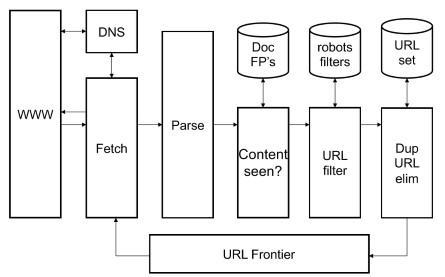
\includegraphics[scale = 1.6]{img/crawler architecture.jpg}
		\label{crawler arch}
        \caption{Architecture of a crawler}
\end{figure}

\begin{enumerate}
    \item The \textbf{URL frontier}, containing URLs yet to be fetched in the current crawl (in the case of continuous crawling, a URL may have been fetched previously but is back in the frontier for re-fetching);
    \item A \textbf{DNS resolution module} that determines the web server from which to fetch the page specified by a URL;
    \item  A \textbf{fetch module} that uses the http protocol to retrieve the web page at a URL;
    \item A \textbf{parsing module} that extracts the text and set of links from a fetched web page;
    \item A \textbf{duplicate elimination module} that determines whether an extracted link is already in the URL frontier or has recently been fetched.
\end{enumerate}

Crawling is performed by anywhere from \textbf{one} to potentially \textbf{hundreds of threads}, each of which loops through the logical cycle in Picture \ref{crawler arch}. These threads may be run in a \textbf{single process}, or be \textbf{partitioned} amongst \textbf{multiple processes} running at different nodes of a distributed system. We begin by assuming that the \textbf{URL frontier} is \textbf{in place} and \textbf{non-empty}. Then, we follow the progress of a single URL through the cycle of being fetched, passing through various checks and filters, then finally (for continuous crawling) being returned to the URL frontier. 

A crawler thread begins by \textbf{taking a URL} from the \textbf{frontier} and fetching the web page at that URL, generally using the \textit{http} protocol. The \textbf{fetched page} is then \textbf{written} into a \textbf{temporary store}, where a number of operations are performed on it. Next, the page is \textbf{parsed} and the text as well as the links in it are extracted: the text is passed on to the indexer, while the link goes through a series of tests to determine whether the link should be added to the URL frontier. 

First, the thread \textbf{tests} whether a \textbf{web page} with the \textbf{same content} has \textbf{already been seen} at another URL: the simplest implementation for this would use a simple fingerprint, while more sophisticated tests would use shingles. Next, a \textbf{URL filter} is used to determine whether the \textbf{extracted URL} should be \textbf{excluded} from the \textbf{frontier} based on one of \textbf{several tests}. For instance, the crawl may seek to exclude certain domains. Notice that a similar test could be \textbf{inclusive} rather than \textbf{exclusive}: many hosts on the Web place certain \textbf{portions} of their \textbf{websites} \textbf{off-limits to crawling}, under a standard known as the \textbf{Robots Exclusion Protocol}. This is done by placing a file with the name \textit{robots.txt} at the root of the URL hierarchy at the site. Here is an example\textit{ robots.txt} file that specifies that no robot should visit any URL whose position in the file hierarchy starts with \textit{/yoursite/temp/}, except for the robot called \textit{“searchengine”}.

\begin{figure}[h!]
		\centering
		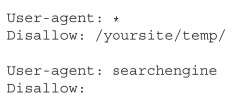
\includegraphics[scale = 1.8]{img/robots.jpg}
		\label{robots}
        \caption{Example of \textit{robots.txt} file}
\end{figure}

Next, a URL should be \textbf{normalized}, and, finally,  the URL is \textbf{checked} for \textbf{duplicate elimination}: if the URL is already in the frontier or (in the case of a non-continuous crawl) already crawled, we do not add it to the frontier. When the URL is added to the frontier, it is assigned a \textbf{priority} based on which it is eventually removed from the frontier for fetching.

\subsubsection{DNS resolution}
Given a URL in textual form, the process of translating it to an IP address is called \textbf{DNS resolution}: during this phase, the component of the web crawler contacts a \textit{DNS server} that returns the translated IP address.

DNS resolution is a well-known \textbf{bottleneck} in web crawling. Due to the \textbf{distributed nature} of the Domain Name Service, DNS resolution may entail \textbf{multiple requests} and round-trips across the internet, requiring seconds and sometimes even longer. Right away, this puts in \textbf{jeopardy} our goal of \textbf{fetching several hundred documents a second}. A standard remedy is to introduce \textbf{caching}: URLs for which we have recently performed DNS lookups are likely to be found in the DNS cache, avoiding the need to go to the DNS servers on the internet. However, obeying politeness constraints limits the of cache hit rate. 

There is another important difficulty in DNS resolution; the \textbf{lookup implementations} in standard libraries (likely to be used by anyone developing a crawler) are generally \textbf{synchronous}. This means that \textbf{once a request is made} to the Domain Name Service, \textbf{other} crawler \textbf{threads} at that node \textbf{are blocked} until the first request is completed. To circumvent this, most web crawlers implement their \textbf{own DNS resolver} as a component of the crawler. 

\subsubsection{URL frontier}
Two important considerations govern the \textbf{order} in which \textbf{URLs} are \textbf{returned by the frontier}:

\begin{enumerate}
    \item \textbf{Freshness}, i.e. \textbf{high-quality pages} that change frequently should be \textbf{prioritized} for \textbf{frequent crawling}. Thus, the \textbf{priority} of a page should be a \textbf{function} of both its \textbf{change rate} and its \textbf{quality} (using some reasonable quality estimate). The combination is necessary because a large number of spam pages change completely on every fetch;
    \item \textbf{Politeness}, i.e. we must \textbf{avoid repeated fetch requests to a host within a short time span}. A common heuristic is to insert a time gap between successive requests to an host.
\end{enumerate}

Clearly, these goals may conflict with each other. 

A state-of-the-art (continuous) web crawler maintains two separate queues for prioritizing the download of URLs:

\begin{itemize}
    \item The \textbf{discovery queue}, which downloads pages that are not previously downloaded, pointed by already discovered links;
    \item The \textbf{refreshing queue}, which re-downloads already downloaded pages, and thus tries to increase the freshness of the repository.
\end{itemize}

Since the Web is dynamic, the general problem is that the client must periodically poll the remote source to detect changes with local copies and refresh them. In general, the \textit{freshness} $F$ and the \textit{age} $A$ of a page $e_i$ are defined as:

$$
F(e_i; t) = \begin{cases}
    1 \qquad \text{if } e_i \text{ is up-to-date at time} t \\
    0 \qquad \text{otherwise}
\end{cases}
$$

$$
A(e_i; t) = \begin{cases}
    0 \qquad \text{if } e_i \text{ is up-to-date at time} t \\
    (t - \text{modification time of } e_i) \qquad \text{otherwise}
\end{cases}
$$

The evolution in time of \textit{freshness} and \textit{age} are represented in Picture \ref{freshness and age}.

\begin{figure}[h!]
		\centering
		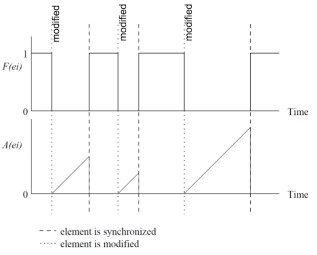
\includegraphics[scale = 1.8]{img/fr and age.jpg}
		\label{freshness and age}
        \caption{Evolution of freshness and age over time}
\end{figure}

In general, the goal of the refreshing operation is to maintain the average number of fresh pages as high as possible, and the average age of the pages as low as possible. In this sense, the update can be either uniform, i.e. regardless of the age of the page, or proportional to the change rate of a page: in a simulated environment, the uniform strategy is surprisingly better, since the crawler wastes a lot of time in trying to keep updated pages changing often, so in order to improve freshness, we must penalize pages changing too often.

\subsubsection{Distributed crawler}

We have mentioned that the threads in a crawler could run under different processes, each at a different node of a distributed crawling system. Such distribution is essential for scaling; it can also be of use in a \textbf{geographically distributed crawler system} where each node crawls hosts “near” it. Partitioning the hosts being crawled amongst the crawler nodes can be done by a hash function, or by some more specifically tailored policy. For instance, we may locate a crawler node in Europe to focus on European domains, although this is not dependable for several reasons.

How do the \textbf{various nodes} of a distributed crawler \textbf{communicate} and \textbf{share URLs}? The idea is to replicate the flow of Picture \ref{crawler arch} at each node, with one essential difference: following the URL filter, we use a \textbf{host splitter} to dispatch each surviving URL to the crawler node responsible for the URL; thus the set of hosts being crawled is partitioned among the nodes. This modified flow is shown in Picture \ref{distr crw}. The output of the host splitter goes into the Duplicate URL Eliminator block of each other node in the distributed system. 

\begin{figure}[h!]
		\centering
		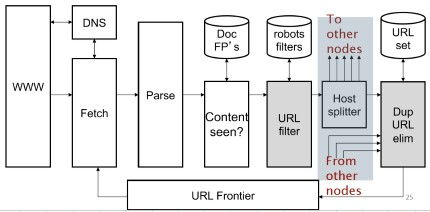
\includegraphics[scale = 1.8]{img/distributed crawler.jpg}
		\label{distr crw}
        \caption{Distributed version of the crawl architecture}
\end{figure}

In this sense, the idea is to assign a partition of the Web to each of the crawlers, and this \textbf{Web partitioning} can be, for example {Hash-based}, i.e. based on the MD5 hashes of either canonical URLs or host names. Moreover, regarding \textbf{fault tolerance}, when a crawling node dies, its URLs are redistributed over the remaining crawler nodes.




